
\documentclass{article}
\usepackage{tikz}
\usetikzlibrary{bayesnet}
\usepackage{amsmath}
\usepackage{algorithm}
\usepackage{algorithmicx}
\usepackage{algpseudocode}
\usepackage{bm}
\usepackage{graphicx}
\usepackage{appendix}

\usepackage{indentfirst} 
\setlength{\parindent}{2em}

\renewcommand{\algorithmicrequire}{\textbf{Arguments:}}
\renewcommand{\algorithmicensure}{\textbf{Outputs:}}  

\begin{document}

\title{Report: Seam Carving as HMM \\ CS5340 Uncertainty Modeling in AI}
\author{Xudong Shen (A0210662R) \& Ruixi Lin (A0210662R)}
\maketitle

\section*{Background}
	Effective image resizing should consider not only geometry but also image content, i.e., content-aware image resizing. Seam carving \cite{SeamCarving} is a simple method, which builds on Hidden Markov Model (HMM), to achieve this. It resizes an image by successively deleting or duplicating a vertical/horizontal seam with lowest energy. In implementation, the optimal seam can be tracked using Viterbi algorithm.

	In this project we only consider the Viterbi algorithm part: given the enregy map of a image, find the vertical seam with minimal energy.

\section*{Problem formulation}
	We construct the Hidden Markov Model as Figure 1. Observed variable $x_{n}, n=1, ..., H$ represents $n^{th}$ row of the image. Latent variable $z_{n}, n=1, ..., H$ represent the seam's pixel's index in each row. Each latent variable $z_{n}$ takes one discrete state from $\{1, 2, ..., W\}$. $H, W$ are the height and width of the image, repectively.

	\begin{figure}[htbp]
	\begin{center}
	    \tikz{ 
	        \node[obs] (x1) {$x_{1}$} ; 
	        \node[latent, above=of x1] (z1) {$z_{1}$} ; 
	        \node[obs, right=of x1] (x2) {$x_{2}$} ; 
	        \node[latent, above=of x2] (z2) {$z_{2}$} ; 
	        \node[obs, right=of x2] (x3) {$x_{3}$} ; 
	        \node[latent, above=of x3] (z3) {$z_{3}$} ; 
	        \node[const, right=of z3] (z4) {$ \quad \ldots \ldots \quad$} ; 
	        \node[latent, right=of z4] (zH) {$z_{H}$} ; 
	        \node[obs, below=of zH] (xH) {$x_{H}$} ; 

	        \edge {z1} {x1} ; 
	        \edge {z2} {x2} ;
	        \edge {z3} {x3} ;
	        \edge {zH} {xH} ;  

	        \edge {z1} {z2} ; 
	        \edge {z2} {z3} ;
	        \edge {z3} {z4} ; 
	        \edge {z4} {zH} ;  
	    }
    \end{center}
    \caption{Graphical model representation of HMM}
    \end{figure}

    The joint probability can be expressed as:
    \begin{equation}
    	p(X|Z) = \prod_{n=1}^{H}p(x_{n}|z_{n})p(z_{n}|z_{n-1})
    \end{equation}

    The states of the latent variables (equivalent to the seam's pixels' indexes) can be found by maximun a posteriori estimation.
    \begin{equation}
    	\underset{z_{i}, i=1, \ldots, H}{\operatorname{argmax}} \prod_{n=1}^{H}p(x_{n}|z_{n})p(z_{n}|z_{n-1})
    \end{equation}

    The state with lower energy corresponds to higher probability of being occupied. We reconstruct eq.(2) in terms of energy. We work on the log probability.
    \begin{equation}
    	\underset{z_{i}, i=1, \ldots, H}{\operatorname{argmin}} \sum_{i=1}^{H} [ln(e(i,z_{i})) + ln(p(z_{i-1},z_{i}))]
    \end{equation}

    where $e(i,z_{i})$ is the energy term of each pixel at $(i,z_{i})$, and $p(z_{i-1},z_{i})$ is the transition probabilty that ensures continuity.

\section*{Viterbi algorithm}
	Optimal seam can be found using Viterbi algorithm. Similar to \cite{SeamCarving}, first we traverse the image from the first row to the last row to calculate the cumulative log probability, according to eq. (4). Upon arriving at the last row, the minimun cumulative log probability gives $z_{H}$, the index of the last pixel of the seam.
	\begin{equation}
    	M(i,z_{i}) = ln(e(i,z_{i})) + min(M(i-1,z_{i}-1), M(i-1,z_{i}), M(i-1,z_{i}+1))
    \end{equation}

    Then, we backtrack to find the seam with the minimun energy.

\section*{Pseudo code}
	See algorithim 1.

	\begin{algorithm}
	    \caption{Viterbi algorithm}
	    \begin{algorithmic}[1]
	    \Require{Energy map $\bm{E}$, Height $H$, Width $W$}
	    \Ensure{seam indexes $\bm{s}$}
	    	\Function{viterbi}{{$\bm{E}$}}
		        \Procedure{Forwardpass}{}
		            \For{$r$ in $range(H)$} \Comment{enumerate rows}
		            	\If{$r$ = $0$} \Comment{initialize first row}
		            		\State $\bm{m}(:) \gets ln(\bm{E}(r,:))$
		            		\State $\bm{m}_{old} \gets \bm{m}$
		            	\Else
		            	\For{$k$ in $range(W)$} \Comment{enumerate all posible states}
		            		\State $\phi(r,k) \gets \underset{i=k-1,k,k+1}{\operatorname{argmin}}\bm{m}_{old}(i)$
		            		\State $\bm{m}(k) \gets ln(\bm{E}(r,z_{i}))+\bm{m}_{old}(\phi(r,k))$ \Comment{accumulate}
		            	\EndFor
		            	\State $\bm{m}_{old} \gets \bm{m}$ \Comment update to next row
		            	\EndIf
		            	\EndFor
		        \EndProcedure
		        \Procedure{Backtrack}{}
		        \For{$r$ in $range(H-1,-1.-1)$} \Comment{enumerate rows reversely}
		        	\If{$r$ = $H-1$} \Comment{find the seam end to start with}
		        		\State $\bm{s}(r) \gets \underset{k}{\operatorname{argmin}}\bm{m}(k)$
		        	\Else \Comment{backtrack seam index}
		        		\State $\bm{s}(r) \gets \phi(r+1,\bm{s}(r+1))$
		        	\EndIf
		        \EndFor
		        \EndProcedure
		    	\State return $\bm{s}$
	        \EndFunction
	    \end{algorithmic}
	\end{algorithm}

\section*{Experiment}
	The input image and its original energy map (note the energy map changes after each seam operation) is shown in Figure 2, both of size 164*111 pixels. In the energy map, darker color indicates higher energy.

	\begin{figure}[htbp]
	\centering
	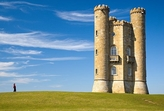
\includegraphics[height=3cm]{input_image.jpg}
	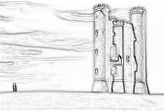
\includegraphics[height=3cm]{original_energy_map.jpg}
	\caption{Input image and its energy map}
	\end{figure}

	In order to better understand the optimal seam, we set the number of seams that need to be carved out as 100 and plot the seam energy. The seam energy is the sum of each pixel's energy. See Figure 3.

	It is worthnoting that, although each seam is of the lowest energy configuration in each image (image changes after preceding operations), it is not guaranteed that preceding seams will be of lower energy tham latter ones.

	\begin{figure}[htbp]
	\centering
	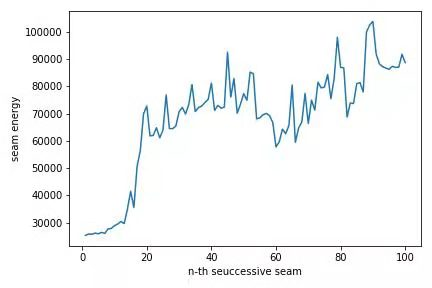
\includegraphics[height=5cm]{seam_energy.jpg}
	\caption{n-th Seam energy}
	\end{figure}

	We also set the number of seams to be carved out as 10, 20, 30, 40, 50, 60, 70, 80, 90, 100, respectively. See Figure 4 for the outputs. It gives an informative visualization of how Seam Carving method carve out the seams successivley.

	\begin{figure}[htbp]
	\begin{tabular}{llll}%
	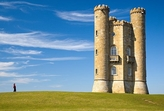
\includegraphics[height=2cm]{input_image.jpg} &
	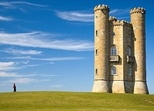
\includegraphics[height=2cm]{image_output_10.jpg} &
	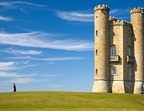
\includegraphics[height=2cm]{image_output_20.jpg} &
	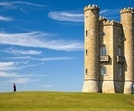
\includegraphics[height=2cm]{image_output_30.jpg} \cr
	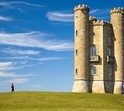
\includegraphics[height=2cm]{image_output_40.jpg} &
	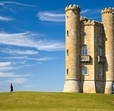
\includegraphics[height=2cm]{image_output_50.jpg} &
	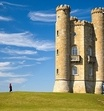
\includegraphics[height=2cm]{image_output_60.jpg} &
	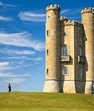
\includegraphics[height=2cm]{image_output_70.jpg} \cr
	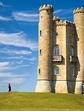
\includegraphics[height=2cm]{image_output_80.jpg} &
	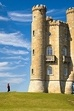
\includegraphics[height=2cm]{image_output_90.jpg} &
	
\includegraphics[height=2cm]{image_output_100.jpg}
	\end{tabular}
	\centering
	\caption{upperleft is the input image. The rest are outputs after deleting different numbers of vertical seams. Images from left to right and from top down corresponds to seam number 10 to 100, respectively.}
	\end{figure}

	Finally, in Figure 5 we set the number of seams to be carved out as 30 and label them in the input image.

	\begin{figure}[htbp]
	\centering
	
\includegraphics[height=5cm]{seams_30.jpg}
	\caption{seams labeled in the input image}
	\end{figure}

\bibliographystyle{unsrt}
\bibliography{./Reference} 

\end{document}











